\documentclass[15pt,a5paper,reqno]{article}
\usepackage{hyperref}
\usepackage[warn]{mathtext}
\usepackage[utf8x]{inputenc}
\usepackage{amssymb, amsmath, multicol}
\usepackage[russian]{babel}
\usepackage{graphicx}
\usepackage[shortcuts,cyremdash]{extdash}
\usepackage{wrapfig}
\usepackage{floatflt}
\usepackage{lipsum}
\usepackage{verbatim}
\usepackage{concmath}
\usepackage{euler}
\usepackage{xcolor}
\usepackage{etoolbox}
\usepackage{fancyhdr}
\usepackage{subfiles}
\usepackage{enumitem}
\usepackage{amsthm}
\usepackage{indentfirst}
\usepackage{import}

\DeclareMathOperator{\sign}{sign}

\RequirePackage[ left     = 1.5cm,
  right    = 1.5cm,
  top      = 2.0cm,
  bottom   = 1.25cm,
  includefoot,
  footskip = 1.25cm ]{geometry}
\setlength    {\parskip}        { .5em plus .15em minus .08em }
%\setlength    {\parindent}      { .0em }
\renewcommand {\baselinestretch}{ 1.07 }

\fancyhf{}

\renewcommand{\footrulewidth}{ .0em }
\fancyfoot[C]{\texttt{\textemdash~\thepage~\textemdash}}
\fancyhead[R]{\hfilШурыгин, Тяжкороб, Широкова}

\makeatletter
\patchcmd\l@section{%
  \nobreak\hfil\nobreak
}{%
  \nobreak
  \leaders\hbox{%
    $\m@th \mkern \@dotsep mu\hbox{.}\mkern \@dotsep mu$%
  }%
  \hfill
  \nobreak
}{}{\errmessage{\noexpand\l@section could not be patched}}
\makeatother
\parindent = 1cm % отступ при красной строке⏎
\pagestyle{fancy}    
\renewcommand\qedsymbol{$\blacksquare$}

\newcommand{\when}[2]{
  \left. #1 \right|_{#2} \hspace
}
\renewcommand{\kappa}{\varkappa}
\RequirePackage{caption2}
\renewcommand\captionlabeldelim{}
\newcommand*{\hm}[1]{#1\nobreak\discretionary{}

\DeclareSymbolFont{T2Aletters}{T2A}{cmr}{m}{it}
{\hbox{$\mathsurround=0pt #1$}}{}}
% Цвета для гиперссылок
\definecolor{linkcolor}{HTML}{000000} % цвет ссылок
\definecolor{urlcolor}{HTML}{799B03} % цвет гиперссылок
 
\hypersetup{pdfstartview=FitH,  linkcolor=linkcolor,urlcolor=urlcolor, colorlinks=true}


%\setcounter{secnum[utf8x]depth}{0}

\begin{document}

% НАЧАЛО ТИТУЛЬНОГО ЛИСТА
\begin{center}
  {\small ФЕДЕРАЛЬНОЕ ГОСУДАРСТВЕННОЕ АВТОНОМНОЕ ОБРАЗОВАТЕЛЬНОЕ\\ УЧРЕЖДЕНИЕ ВЫСШЕГО ОБРАЗОВАНИЯ\\ МОСКОВСКИЙ ФИЗИКО-ТЕХНИЧЕСКИЙ ИНСТИТУТ\\ (НАЦИОНАЛЬНЫЙ ИССЛЕДОВАТЕЛЬСКИЙ УНИВЕРСИТЕТ)\\ ФИЗТЕХ-ШКОЛА РАДИОТЕХНИКИ И КИБЕРНЕТИКИ}\\
  \hfill \break
  \hfill \break
  \hfill \break
  \Huge{Операционные усилители}\\
\end{center}

\hfill \break
\hfill \break
\hfill \break
\hfill \break
\hfill \break
\hfill \break

\begin{flushright}
  \normalsize{Работу выполнили:}\\
  \normalsize{\textbf{Шурыгин Антон Алексеевич, группа Б01-909 \\
                      Тяжкороб Ульяна Владимировна, группа Б01-909   \\   
                      Широкова Ксения Михайловна, группа Б01-909}}\\
\end{flushright}

\begin{center}
  \normalsize{\textbf{Долгопрудный, 2021}}
\end{center}


\thispagestyle{empty} % выключаем отображение номера для этой страницы

% КОНЕЦ ТИТУЛЬНОГО ЛИСТА

\newpage
\thispagestyle{plain}
\tableofcontents
\thispagestyle{plain}
\newpage


\section{Измерение коэффициента усления ОУ}

    $R_1 = R_2 = R_3 = 100$кОм;
    $R_4 = 1$кОм

    \vspace{0,3cm}

    $U_{in} = 3$В;
    $f = 20$Гц

    \vspace{0,3cm}

    Измеренные : $U_a = 12.9$мВ; $U_{out} = 564.6$мВ

    \vspace{0,3cm}

    $A_0 = (1 + \frac{R_3}{R_4}) * \frac{U_{out}}{U_{in}} = 19,0082$

\section{Амплитудно-частотная характеристика ОУ}
    Зависимость коэффициента усиления от частоты (АЧХ):
    $$ A(f) = \frac{U_{out}}{U_{in}} = \frac{U_{out}}{U_{in}} * \frac{U_a}{U_d} = (1 + \frac{R_3}{R_4}) * \frac{U_{out}}{U_a}$$
    \begin {figure}[h!]
      \center{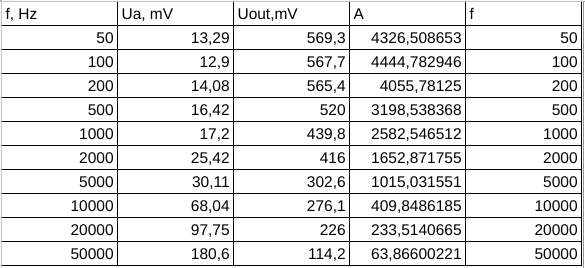
\includegraphics[width = 12cm]{pictures/2_1.png}}
      \caption{Таблица амплитудно-частотной хар-ки ОУ}      
      \label {fig:image1}
    \end {figure}

    \begin {figure}[h!]
    \center{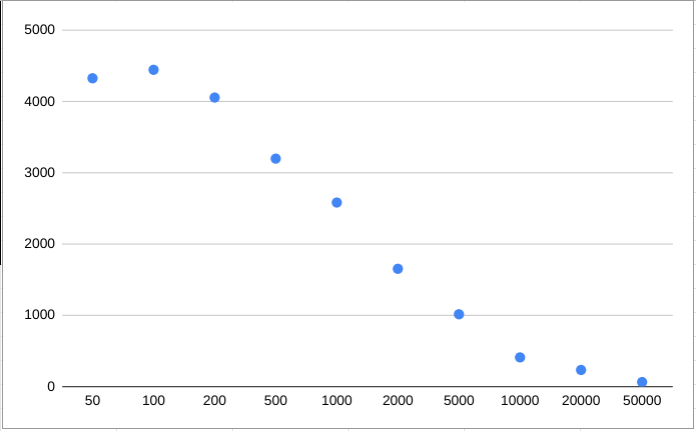
\includegraphics[width = 12cm]{pictures/2_1graph.png}}\\
      \caption{Зависимость A(f)}
    \label {fig:image2}
    \end {figure}

    \begin {figure}[h!]
      \center{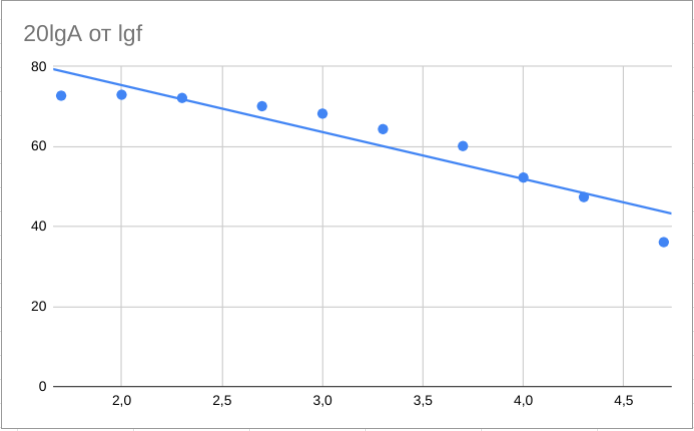
\includegraphics[width = 12cm]{pictures/2_2graph.png}}\\
      \caption{Зависимость 20lgA(lgf)}
      \label {fig:image3}
    \end {figure}


\section{Неинвертирующий усилитель}

Собираем схему с параметрами $R_2 = 10$ кОм, $R_1 = 1$ кОм.

1) Измеряем напряжение постоянного сдвига $U_{OS}$. 

Для этого измеряем постоянное напржение на выходе.

\[ U_{out} = 69 mV \]

\[  U_{OS} = \frac{U_{out}}{1 + \frac{R_2}{R_1}} \approx 6.27 mV \]


2) Снимем зависимость коэффициента усиления от частоты и занесём данные в таблицу:

\begin {figure}[h!]
      \center{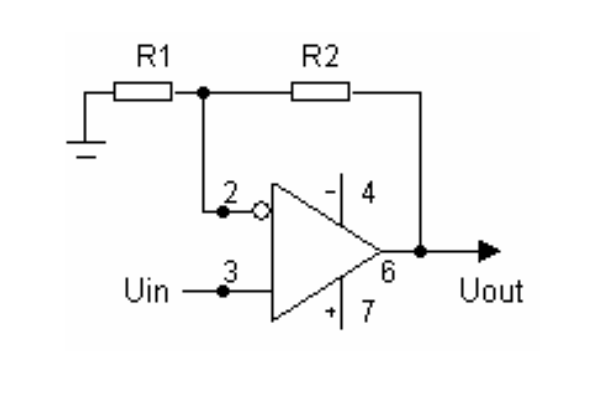
\includegraphics[width = 8cm]{pictures/non_invert_oU.png}}
      \caption{Схема Неинвертирующего ОУ}      
      \label {fig:image1}
\end {figure}

\begin {figure}[h!]
      \center{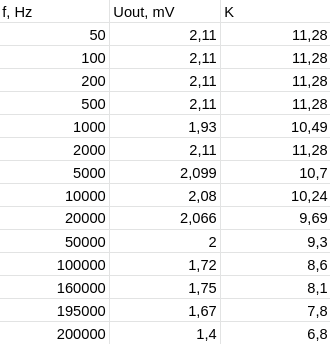
\includegraphics[width = 8cm]{pictures/table_3.png}}
      \caption{Заисимость кэффициента усиления от частоты}      
      \label {fig:image1}
\end {figure}

\begin {figure}[h!]
      \center{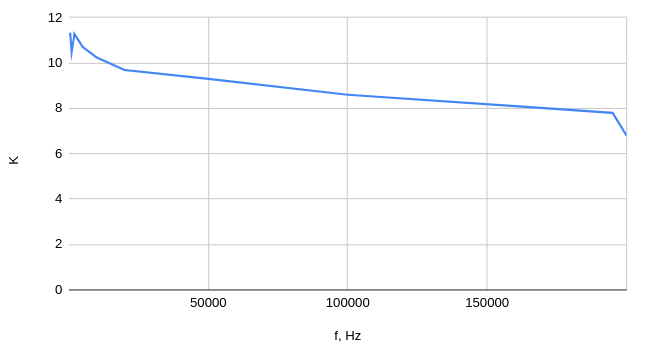
\includegraphics[width = 12cm]{pictures/graph3.png}}
      \caption{Заисимость кэффициента усиления от частоты}      
      \label {fig:image1}
\end {figure}

3)Из таблицы 2 определяем граничную частоту $F_p$ по уровню 0.7:

\[  F \approx 160000 \: Hz     \] 

4)Рассчитаем:

\begin{equation}
    \beta = \frac{R_1}{R_1 + R_2} \approx 0.09
\end{equation}

5)Измерим величину $f_t$ - частоту, на которой $K \approx 1$.

\[  f_t \approx 1.7 \: MHz \]

Из графика видно, что на низких частотах $K_0 \approx 10$. 
Отсюда получаем, что, что действительно $K_0 \approx 11 $.

6) Кроме того, получаем, что $F_p \approx \beta \cdot f_t = 0.9 \cdot 1.7 \: MHz$ действительно выполняется.

7) Включим ОУ по схеме повторителя, т.е $R_1 = \infty, \: R_2 = 0$.
Коэффициент передачи $K = 1$.


Измерим на частоте $f = 0.5 − 1$ МГц максимальную амплитуду неискажённого сигнала, получим $U_{max} = 1.15$ В. Рассчитаем её теоретическое значение по следующей
формуле:

\[ U_{m_{out}} = \frac{V_{max}}{2 \pi f}  \]

Действительно, $U_{m_{out}} \approx 0. 73 \approx 1$.

Полученное экспериментальное довольно хорошо близко к теоретическому.

Учитывая полученное $U_{max} = 1.15$ В, а так же $V_{max} = 3 \frac{В}{мкс}$.


\section{Инвертирующий усилитель}


\begin {figure}[h!]
      \center{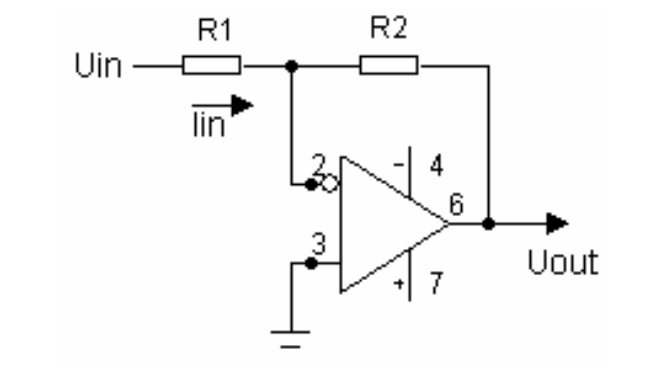
\includegraphics[width = 6cm]{pictures/invert_oU.png}}
      \caption{Cхема инвертирующего усилителя}      
      \label {fig:image1}
\end {figure}

1) Соберём схему с теми же резисторами, что и в предыдущем пункте.
Определим коэффициент усиления $K_0 \approx −11$.

Граничная частоту $F_p = 160 \: KHz$. 

Заметим, что $K_0 = -\frac{R_2}{R_1}$, а частота $F_p \approx 160 KHz$ имеет то же значение, что и в предыдущем пункте.

\end{document}
